\begin{comment}
%%%%%%%%%%%%%%%%%%%%%%%%%%%%%%%
\section{Grover's algorithm} \label{Grover-section}
%%%%%%%%%%%%%%%%%%%%%%%%%%%%%%%


One of the earliest algorithms that was designed to use quantum resources is described in a 1996 paper by Lov Grover \cite{grover1996}. The algorithm attempts to solve the following problem: imagine you have a database of elements. We can represent them as bit strings, but we know that one of them is `marked' by some function acting on that bit string. Examining the case where we have 4 numbers (2 bits), we have the following truth table. 

\begin{equation}
\begin{array}{c|c|c}
    & x & f(x) \\
    \hline
    0 & 00 & 0 \\
    1 & 01 & 0 \\
    2 & 10 & 1 \\
    3 & 11 & 0 \\
\end{array}
\end{equation}

This unstructured search is an important problem in computer science. If we used a classical computer to try to find the marked element `10' above we'd have to try at least 3 times, since we could always end up with it being the last element applied to f(x). This scales as expected, so we can write that at worst it takes N attempts to find the marked element, which can be written O(N).

However, using the principle of superposition, we can explore the whole space of elements simultaneously. To do this we need two matrices (or gates): one which is a diagonal matrix with $(-1)^{f(x)}$ as its elements. For the marked element being 10 as above, we have

\begin{align}
        U_f = \begin{pmatrix}
        1 & 0 & 0 & 0 \\
                 0 & 1 & 0 & 0\\
                 0  & 0 & -1 & 0 \\
                 0 & 0 & 0 & 1
        \end{pmatrix}
\end{align}

The second ingredient is the following matrix, (irrespective of which element is marked).

\begin{align}
        D = \frac{1}{2}\begin{pmatrix}
        -1 & 1 & 1 & 1 \\
                 1 & -1 & 1 & 1\\
                 1  & 1 & -1 & 1 \\
                 1 & 1 & 1 & -1
        \end{pmatrix}
\end{align}

Now we will look at the algorithm step-by-step for this simple four element (two qubit) case. Starting with the qubits in the `00` state, we generate a superposition using a so called Hadamard gate (represented by H) on each qubit, which takes $00 \rightarrow 00 + 01 + 10 +11$ (we have ignored normalisation for simplicity). This can be represented by the matrix transformation

\begin{align}
        \frac{1}{2}
        \begin{pmatrix}
        1 & 1 & 1 & 1 \\
        1 & -1 & 1 & -1\\
        1  & 1 & -1 & -1 \\
        1 & -1 & -1 & 1
        \end{pmatrix}
        \begin{pmatrix}
        1\\
        0\\
        0\\
        0\\
        \end{pmatrix}
        =
        \frac{1}{2}
        \begin{pmatrix}
        1\\
        1\\
        1\\
        1\\
        \end{pmatrix}
\end{align}

In the next step of the algorithm, we apply $U_f$. This picks out the marked element, giving it a minus sign and adding a $\pi$ phase shift to the other elements.

\begin{align}
        \frac{1}{2}
        \begin{pmatrix}
        1 & 0 & 0 & 0 \\
        0 & 1 & 0 & 0\\
        0  & 0 & -1 & 0 \\
        0 & 0 & 0 & 1
        \end{pmatrix}
        \begin{pmatrix}
        1\\
        1\\
        1\\
        1\\
        \end{pmatrix}
        =
        \frac{1}{2}
        \begin{pmatrix}
        1\\
        1\\
        -1\\
        1\\
        \end{pmatrix}
\end{align}

The final step is to apply $D$. The construction is $D$ is such that each row, when multiplied by the vector, converts the $\pi$ phase difference into unit value . This can be thought of as a constructive interference on the marked element instead of destructive interference on all of the other elements. 

\begin{align}
    \frac{1}{2}.\frac{1}{2}
    \begin{pmatrix}
    -1 & 1 & 1 & 1\\
    1 & -1 & 1 & 1 \\
    1 & 1 & -1 & 1 \\
    1 & -1 & -1 & 1 \\
    \end{pmatrix}
    \begin{pmatrix}
    1 \\ 1 \\ -1 \\ 1 
    \end{pmatrix}
    =
    \frac{1}{4}
    \begin{pmatrix}
    0 \\ 0 \\ 4 \\ 0
    \end{pmatrix}
    = 
    \begin{pmatrix}
    0 \\ 0 \\ 1 \\ 0
    \end{pmatrix}
\end{align}

From this we can see that the general recipe of Grover's algorithm is to create a superposition of all the possible states, add a $\pi$ phase shift to the marked states with the special unitary $U_f$, and then use $D$ to pick out this phase shift.

In this case the algorithm has successfully found the marked element with certainty (though this does not take into account any experimental imperfections observed in real life). However, using superpositions inevitably leads to success with a non-unity success rate, as demonstrated in the next section, where we look at the three qubit case described using Dirac notation instead of matrices, as now we would have to use $8\times8$ matrices - this demonstrates the exponential scaling that quantum computing demonstrates, with $2^n\times2^n$ matrices being required for $n$ qubits. Hence the transition to Dirac notation is quite a natural progression to larger system sizes. 

%%%%%%%%%%%%%%%%%%%%%%%%%%%%%%%%%%%%%%%%%
\subsubsection{Alternative representation: Dirac notation}
Here we consider a problem on $N=8$ elements, where the fifth element is marked. The algorithm can be applied with a minimum of $3$  ($2^{3}=8$) qubits in the following manner:

\begin{tcolorbox}[standard jigsaw,
    opacityback=0,  % this works only in combination with the key "standard jigsaw"
    boxrule=0.5pt,label={example100100000}]
    {\bf Grover's Algorithm}
    \tcbline
    \begin{enumerate}
    \item Start with the state $\ket{000}$.
    \item Apply the Hadamard gates which result in the state: $\ket{\Psi}=\dfrac{1}{2\sqrt{2}}\big(\ket{000}+\ket{001}+\ket{010}+\ket{011}+\ket{100}+\ket{101}+\ket{110}+\ket{111}\big)$
    \item Apply $U_{f}$, which reverses the sign on the fifth element: $\ket{\Psi}=\dfrac{1}{2\sqrt{2}}\big(\ket{000}+\ket{001}+\ket{010}+\ket{011}-\ket{100}+\ket{101}+\ket{110}+\ket{111}\big)$
    \item Apply D, which leads to state $\ket{\Psi}=\dfrac{1}{4\sqrt{2}}\big(\ket{000}+\ket{001}+\ket{010}+\ket{011}+5\ket{100}+\ket{101}+\ket{110}+\ket{111}\big)$
    \item Repeat steps 3 and 4 ``$T$'' times, where $T$ is to be determined later.
    \item Measure the state $\ket{\Psi}$.
    \end{enumerate}
\end{tcolorbox}



\begin{figure}
    \centering
    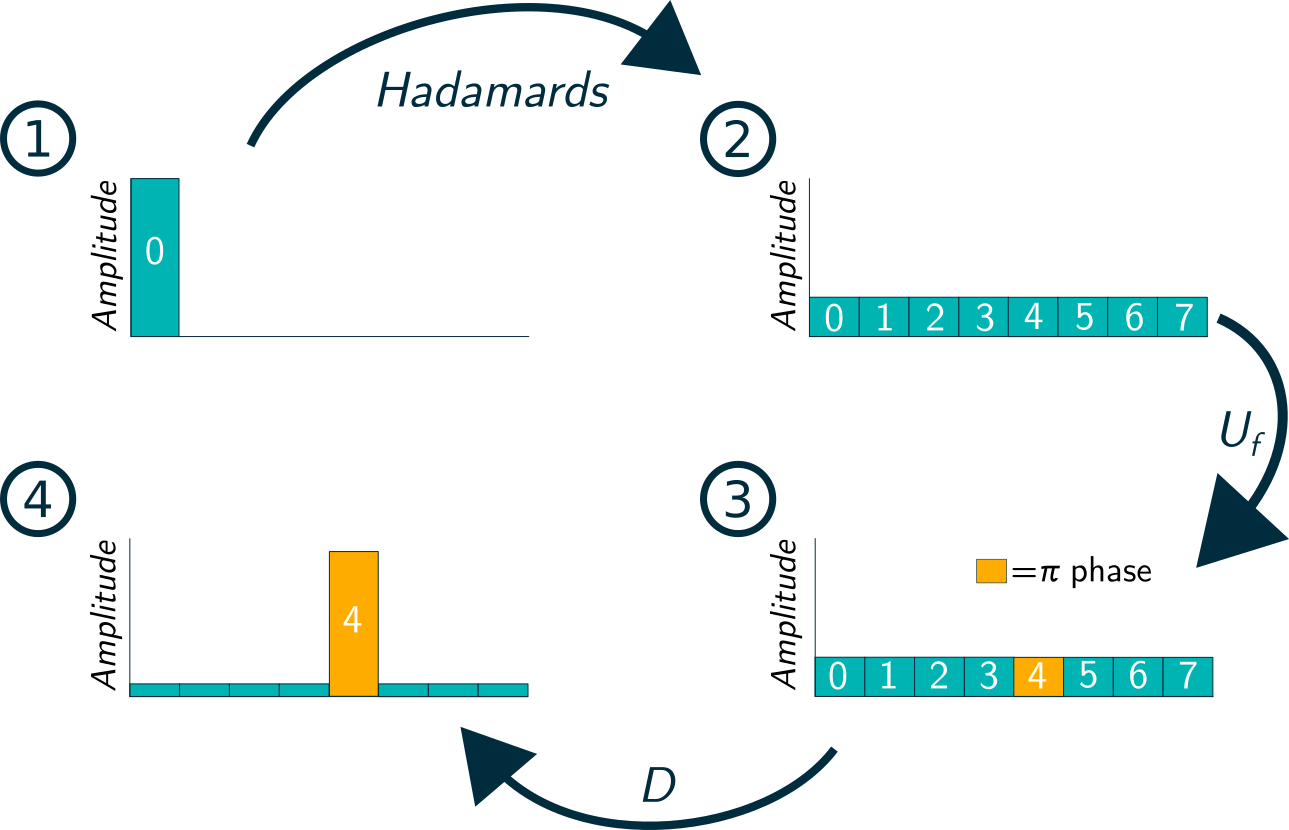
\includegraphics[width=0.9\linewidth]{figures/Grovers.png}
    \caption{Pictorial demonstration of the steps of Grover's Algorithm}
    \label{fig:Grovers}
\end{figure}


In the step 2 above, applying the Hadamard gate to all the qubits leads to a state which is in superposition of all possible states (elements). It is important to start with the state $\ket{000}$ so that all the states in the superposition have the same initial phase. In step 3 we apply the $U_{f}$ gate which is dependent on $f(x)$ and is able to recognise the marked element. The oracle applies a $\pi$ phase shift to the marked element but leaves all the other states unchanged. The next step is to apply gate $D$. The application of gate $D$ can be understood as an operation which increases the amplitude of the phase shifted element in step 3, suppressing the amplitude of the others. As mentioned in chapter 1, the measurement of a state leads to an output with a probability equal to the amplitude squared and thus, increasing the amplitude of the marked element state results in a higher probability of a measuring returning that state. It is worth noting that repeating steps 3 and 4 a fixed number of times will increase the probability of detecting the marked element but after a certain point, the probability will start to decrease. For clarification, if we carry out another iteration of steps 3 and 4 in the above example, we get the state:
\begin{align}
\ket{\Psi}=\dfrac{-1}{8\sqrt{2}}\big(\ket{000}+\ket{001}+\ket{010}+\ket{011}-11\ket{100}+\ket{101}+\ket{110}+\ket{111}\big).
\end{align}
 Now if a measurement is performed on this state, there is a 94.53\% chance of getting the fifth element compared to 78.12\% probability after just one iteration. If yet another iteration of step 3 and 4 is performed, the resulting state becomes:

\begin{align}
\ket{\Psi}=\dfrac{-7}{16\sqrt{2}}\big(\ket{000}+\ket{001}+\ket{010}+\ket{011}-\frac{13}{7}\ket{100}+\ket{101}+\ket{110}+\ket{111}\big)    
\end{align}
and the probability of getting the marked element upon measurement decreases further to 67\%. Therefore, it is important to choose the number of iterations for Grover's algorithm carefully. The number of iterations ``$T$'' required to get the maximum probability of measuring the marked element is approximately given by:

\begin{equation}\label{groverIteration}
    T=\big(\pi\big/4)\sqrt{N}
\end{equation}


%%%%%%%%%%%%%%%%%%%%%%%%%%%%%%%%%%%%
\subsubsection{General n-qubit case}

Given a function $f: \left\{0,1\right\}^n \rightarrow \left\{0,1\right\}$ with the promise that $f(x_0) = 1$ for a unique element $x_0$, the problem is to find this $x_0$. We use a quantum circuit on $n$ qubits in the initial state $\ket{0}^{\otimes n}$. Let $H$ denote the Hadamard gate, and let $U_0$ denote the $n$-qubit operation which inverts the phase of $\ket{0^n}$: $U_0\ket{0^n} = -\ket{0^n}$, $U_0\ket{x} = \ket{x}$ for all $x \neq 0^n$. The first step of the algorithm is to apply the Hadamard gate on all $n$ qubits to form the superposition state required for quantum parallel computing. Next, repeat the following operations T times for some T determined by Equation \ref{groverIteration}.
%\begin{enumerate}
%\item Apply $H^{\otimes n}$.

%\item Repeat the following operations T times, for some T to be determined later:
\begin{enumerate}
\item Apply $U_f$, where $U_f\ket{x} = (-1)^{f(x)}\ket{x}$.
\item Apply $D$, where $D = -H^{\otimes n}U_0H^{\otimes n}$
\end{enumerate} 
%\item Measure all the qubits and output the result.
%\end{enumerate}
%\end{tcolorbox}
Finally, measure all the qubits and output the result.\\

In circuit diagram form, Grover's algorithm appears like: \\
\begin{equation*}
\Qcircuit @C=2.14em @R=1.25em
{\lstick{\ket{0}} & \gate{H} & \multigate{5}{U_f} & \multigate{5}{D} & \multigate{5}{U_f} & \ghost{U_f} & \lstick{\dots} & \multigate{5}{D} & \meter \\
\lstick{\ket{0}} & \gate{H} & \ghost{U_f} & \ghost{D} & \ghost{U_f} & \ghost{U_f} &\lstick{\dots} & \ghost{D} & \meter \\ 
& \dot{} & & & & & & & \dot{} \\
& \dot{} & & & & & & & \dot{} \\
& \dot{} & & & & & & & \dot{} \\
\lstick{\ket{0}} & \gate{H} & \ghost{U_f} & \ghost{D} & \ghost{U_f} & \ghost{U_f} & \lstick{\dots} & \ghost{D} & \meter \\}
\end{equation*}

\subsubsection{Construction of gate $D$ and $U_{f}$}
The gate $D$ in the algorithm applied on $n$-qubits can be implemented in the following manner. This shows that gate $D$ requires $2n+1$ Hadamard ($H$) gates, $2n+1$ Pauli $X$ gates and an n-control Toffoli gate.

\begin{align*}
\Qcircuit @C=1.14em @R=1.25em
{\lstick{\ket{x_1}} & \gate{H} & \gate{X} &  \ctrl{1} & \gate{X} & \gate{H} & \qw  \\
\lstick{\ket{x_2}} & \gate{H} & \gate{X} &  \ctrl{4} & \gate{X} & \gate{H} & \qw  \\
\lstick{\dot{}} & \dot{} & \dot{} & & \dot{} & \dot{} & \\
\lstick{\dot{}} & \dot{} & \dot{} & & \dot{} & \dot{} & \\
\lstick{\dot{}} & \dot{} & \dot{} & & \dot{} & \dot{} & \\
\lstick{\ket{x_n}} & \gate{H} & \gate{X} &  \ctrl{1} & \gate{X} & \gate{H} & \qw  \\
\lstick{\ket{0}} & \gate{x} & \gate{H} &  \targ & \qw & \qw & \qw }
\end{align*}

\vspace{1cm}
The construction of gate $U_{f}$ depends upon the function $f(x)$ being addressed by the algorithm.

\end{comment}
%%%%%%%%%%%%%%%%%%%%%%%%%%%%%%%%%%%%%%%%%
\section{Implementing Grover's algorithm}
%%%%%%%%%%%%%%%%%%%%%%%%%%%%%%%%%%%%%%%%%

In this section we will implement Grover's algorithm as discussed in \autoref{Grover-section}. The steps that we need to implement Grover's algorithm are as follows

\begin{enumerate}
    \item{Import/initialise libraries}
    \item{Create the equal superposition}
    \item{Define the oracle operations $U_f$ and $D$ described in \autoref{Grover-section} }
    \item{Perform the oracle operations T times}
    \item{Measure the register to obtain the output}
\end{enumerate}

For our implementations the unique bit string to be found is given by either the user or a random number generator, rather than being given a black box with a single marked element. Therefore this just serves as a simple example for how Grover's algorithm will work.

We will aim to discuss the most important sections of the code which are the quantum parts. For the full code listings please check out our Appendix/Github.

%%%%%%%%%%%%%%%%%%%%%%%%%%%%%%%%%%%%%%%%%%%
%%%%%%%%%%%%%%%%%%%%%%%%%%%%%%%%%%%%%%%%%%%
\subsection{Grover's Algorithm with pyQuil}
%%%%%%%%%%%%%%%%%%%%%%%%%%%%%%%%%%%%%%%%%%%
%%%%%%%%%%%%%%%%%%%%%%%%%%%%%%%%%%%%%%%%%%%

\subsubsection{Initialise libraries}

We start by calling the libraries that we are going to use

\inputminted[lastline=5]{python}{code/pyQuil/grover_pyquil_guide.txt}

and initialise the program

\inputminted[firstnumber=18, firstline=18, lastline=20]{python}{code/pyQuil/grover_pyquil_guide.txt}

\subsubsection{Create the equal superposition}

We can create the equal superposition by looping through all of the qubits and applying a Hadamard to each of them.

\inputminted[firstnumber=22, firstline=22, lastline=24]{python}{code/pyQuil/grover_pyquil_guide.txt}

\subsubsection{Create the oracle operations}

Defining the Oracles matrices and adding them to be gates
\begin{minted}[firstnumber=17]{python}
# Defining Oracle matrices: U0 and Uf
vec0=np.ones((2**n,), dtype=np.int)
vecf=np.ones((2**n,), dtype=np.int)
vec0[0]=vec0[0]*(-1)
vecf[nf]=vecf[nf]*(-1)
U0ma=(-1)*np.diag(vec0) 
Ufma=np.diag(vecf) 
# Defining Oracle gates
p.defgate("U0",U0ma)
p.defgate("Uf",Ufma)
\end{minted}

\subsubsection{Apply the oracle operations}

Calculating T and applying the operator of interest T times.
\begin{minted}[firstnumber=27]{python}
# Calculating T for the loop
T=((np.pi/4)*(1/np.arcsin(1/np.sqrt(2**n))))-0.5 # N=2**n
T=np.rint(T)
T=int(T)
# Applying Oracle loop T times
for i in range(1,T+1,1):
    p.inst(("Uf",)+tuple(range(n)))
    for ii in range(0, n, 1):
        p.inst(H(ii))
    p.inst(("U0",)+tuple(range(n)))
    for ii in range(0, n, 1):
        p.inst(H(ii))
\end{minted}

\subsubsection{Measure the register to obtain the output}

Measuring all the qubits and running the program.
\begin{minted}[firstnumber=39]{python}
# Measurement stage
for ii in range(0, n, 1):
    p.measure(ii,ii)
# Running the program
results=qvm.run(p,[],5)
guess=results[0]
print("""Grover's algorithm is guessing that the marked string is""",guess)
\end{minted}
The algorithm ends up printing a guess for the single-marked string.

%Define it as a function, so that if u run the algorithm it outputs this and that.

%%%%%%%%%%%%%%%%%%%%%%%%%%%%%%%%%%%%%%%%%%%
\subsection{Grover's Algorithm with QISKit}

\subsubsection{Initialise libraries}

Firstly, as with most regular programming languages, we need to import the libraries that we intend to make use of:

\begin{minted}{python}
# Program written using QISKit to demonstrate the way in which to implement Grovers search 
# algorithm and then simulate the measurement on IBM's Q QASM simulator

# Import relevant library functions from QISKit
from qiskit import ClassicalRegister, QuantumRegister, QuantumCircuit, QuantumProgram
from qiskit import available_backends, execute

# Import relevant library functions 
import numpy as np
\end{minted}

Here we define out function, the length of the marked element inputted by the user, the length of said marked element, and the number of qubits required to preform a search algorithm that will find said marked element:

\begin{minted}[firstnumber=10]{python}
def grover(marked_element):
	
	# Determine the number of qubits needed
	n = len(marked_element)
	N = 2**n
	print('Number of Qubits required is', n)
	print('Number of Ancillas required is', n)
\end{minted}

Due to the way in which QISKit handles inputted strings, for the output of our function to make sense it is necessary to flip the values of the use inputted bit string:

\begin{minted}[firstnumber=17]{python}	
	# Flip bitstring
	marked_element = marked_element[::-1]
\end{minted}

Here we add in protection against user input that would require too many qubits to execute successfully. Via QISKit's local Q QASM simulator, we have the equivalent of 32 qubits available to us to preform simulations. In these lines the function returns 0 is the used input requires more than 32 qubits:

\begin{minted}[firstnumber=19]{python}	
	# Check if we can simulate on our local simulator (QASM Local simulator has 32 
	# qubits)
	if n > 32:
		print('Number of qubits required =', 2*n, 'which is too large to simulate.')
		return 0
\end{minted}

The code here shows how we calculate the number of iterations necessary to identify the user inputted bit string:

\begin{minted}[firstnumber=24]{python}	
	# Determine the number of times to iterate 
	T = int(round(np.pi*np.sqrt(N)/4 - 0.5)) 
	print('Number of iterations T =',T)
\end{minted}

Now comes the QISKit element. Below we show how to define our $n$-qubit register, an $n+1$ classical readout register, $n-1$ ancilla qubits for two qubit operations, and a target register to aid in the implementation of an $n$-qubit CNOT gate. We then combine all of these resources into a single quantum circuit we can manipulate:

\begin{minted}[firstnumber=27]{python}
	# Initialise n qubit register, classical readout register and ancilla qubit
	q = QuantumRegister(n, 'ctrl')
	c = ClassicalRegister(n+1, 'meas')
	a = QuantumRegister(n-1, 'anc')
	t = QuantumRegister(1, 'tgt')
	
	# Combine resources into a quantum circuit
	qc = QuantumCircuit(q, a, t, c)
\end{minted}

\subsubsection{Create the equal superposition}

Here we manipulate entire registers by looping through and applying unitary gates to each qubit in the register:

\begin{minted}[firstnumber=35]{python}
	# Step 1: Start in an equal weighted superposition state on the quantum register 
	for i in range(n):
		qc.h(q[i])
	
	# Put the ancilla qubit into the - state
	qc.x(a[0])
	qc.h(a[0])
\end{minted}

\subsubsection{Apply the oracle operations}

From any quantum computation literature it is known that to execute Grover's successfully, the operations $D$ and $U_{f}$ must be repeated sequentially $T$ times. This is shown in the framework of QISKit below:

\begin{minted}[firstnumber=42]{python}	
	# Step 2: Repeat applications of U_f and D
	for i in range(T):
		# Apply U_f 
		for j in range(n):
			if marked_element[j] == '0':
				qc.x(q[j])	
		
		# Implement an n-qubit CNOT gate
		qc.ccx(q[0], q[1], a[0])
		for i in range(2, n):
			qc.ccx(q[i], a[i-2], a[i-1])
		# Copy
		qc.cx(a[n-2], t[0])
		# Uncompute
		for i in range(n-1, 1, -1):
			qc.ccx(q[i], a[i-2], a[i-1])
		qc.ccx(q[0], q[1], a[0])
		
		for j in range(n):
			if marked_element[j] == '0':
				qc.x(q[j])
		
		# Apply D
		
		# Apply H
		for j in range(n):
			qc.h(q[j])
			qc.x(q[j])
		
		# Apply U_0
		# Implement an n-qubit CNOT gate
		qc.ccx(q[0], q[1], a[0])
		for i in range(2, n):
			qc.ccx(q[i], a[i-2], a[i-1])
                # Copy
		qc.cx(a[n-2], t[0])
                # Uncompute
		for i in range(n-1, 1, -1):
			qc.ccx(q[i], a[i-2], a[i-1])
		qc.ccx(q[0], q[1], a[0])
		
		# Apply H
		for j in range(n):
			qc.x(q[j])
			qc.h(q[j])
\end{minted}

\subsubsection{Measure the register to obtain the output}

Coming to the end of the program, we 'measure' our quantum register onto a classical register:

\begin{minted}[firstnumber=87]{python}	
		# Measure our quantum register via our classical register
		for i in range(n):
			qc.measure(q[i], c[i])
\end{minted}

Finally, we execute our program on the local Q QASM simulator:

\begin{minted}[firstnumber=90]{python}
		# Execute the quantum circuit on the local simulator
		job = execute(qc, 'local_qasm_simulator')
		result = job.result()
		print('The results of the simulation shots are:', result.get_counts(qc))
\end{minted}

Here we end the function by defining what type of input the user can submit to the function we just defined:

\begin{minted}[firstnumber=94]{python}
# Define input type for def
str_input = input("Input a bit string to find: ")
grover(str_input) 
\end{minted}

%%%%%%%%%%%%%%%%%%%%%%%%%%%%%%%%%%%%%%%%%%%
\subsection{Grover's Algorithm with ProjectQ}
%%%%%%%%%%%%%%%%%%%%%%%%%%%%%%%%%%%%%%%%%%%

The first thing to do is to import the functions from ProjectQ that will be required to create and run the program.

\inputminted[firstnumber=3, firstline=3, lastline=5]{python}{code/ProjectQ/grover_projectq_guide.txt}

Since ProjectQ is run on a local simulator, your computer, it is good practice to make sure that the number of qubits required for the computation can actually be simulated to avoid crashing the computer. Most modern computers have 8GB of RAM which is exactly enough memory for 29 qubits, but there are other processes being run on the computer so you would only be able to simulate 28.

\inputminted[firstnumber=13, firstline= 13, lastline=16]{python}{code/ProjectQ/grover_projectq_guide.txt}

Now the local simulator can be loaded by calling \texttt{MainEngine} and our qubits allocated. The number of qubits required is the length of the bit string provided by the user plus an ancilla qubit. The ancilla is required because we will use it to implement the oracle $U_f$ and the gate $D$.

\inputminted[firstnumber=22, firstline=22, lastline=25]{python}{code/ProjectQ/grover_projectq_guide.txt}

The main qubits need to start in an equal superposition, so Hadamards can be applied to all of them using the function \texttt{All}. The ancilla needs to start in the $\ket{-}$ state, and since qubits are initialised as $\ket{0}$, we can achieve this with an $X$ followed by a $H$ gate.

\inputminted[firstnumber=27, firstline=27, lastline=30]{python}{code/ProjectQ/grover_projectq_guide.txt}

Now we come to the part of the algorithm where we must alternate between the gates $U_f$ and $D$ for $T$ iterations where $T$ is the closest integer to $\frac{\pi}{4}\sqrt{N} - \frac{1}{2}$. ProjectQ does allow you to define new gates from their matrix representations using \texttt{BasicGate}, but this only works well for one or two qubit gates. Therefore we need a different, more efficient way of doing the oracle. 

To perform $U_f$, we can use the function \texttt{Control} from ProjectQ. This controls on all the qubits being in the state $\ket{1}$ - so it essentially functions as a quantum \texttt{if} statement. Suppose that the marked bit string is '101', $U_f$ should flip the phase of $\ket{101}$. But since we can only control on all the bits being '1', we need to flip the second bit using an $X$ gate. Once we have done this, we can use an $X$ gate on the ancilla to introduce this phase, then flip the second bit back to normal. Our code can now generalise to any bit string.

\inputminted[firstnumber=34, firstline=34, lastline=42]{python}{code/ProjectQ/grover_projectq_guide.txt}

Now we can do a similar construction to implement the gate $D = H^{\otimes n} U_0 H^{\otimes n}$. This time flipping all the qubits with $X$ since we need to control on all the qubits being $\ket{0}$. 

\inputminted[firstnumber=43, firstline=43, lastline=52]{python}{code/ProjectQ/grover_projectq_guide.txt}

Finally, after we exit the loop, we must measure all the qubits using the \texttt{Measure} command and use \texttt{flush} to send all the instructions to the simulator. The result can then be converted to an integer from a qubit type using \texttt{int} and displayed as a string.

\inputminted[firstnumber=54, firstline=54, lastline=59]{python}{code/ProjectQ/grover_projectq_guide.txt}

An example of the input and output is shown below. Up until around 16 qubits, the code takes less than a minute to run. Beyond that, not only do we have more qubits to simulate, but we also have to apply more gates as the number of iterations required increases. For example, trying to find a 20-bit string takes around 30 minutes.

\begin{minted}{python}
Input a bit string to find: 10101
Number of iterations T = 4
Element found = 10101
\end{minted}

%%%%%%%%%%%%%%%%%%%%%%%%%%%%%%%%%%%%%%%%%%%%
\subsection{Grover's Algorithm with Q\#}

We start Grover's algorithm as any other Q\# program, by declaring the namespace we are working in, \texttt{Quantum.Grover} and open the namespaces we will be using.

\lstinputlisting[language=Qsharp, firstnumber=1, linerange={1-7,127-127}]{code/Qsharp/Grover/Grover.txt}

Programming quantum algorithms

When implementing a quantum program, an important step is to check the individual gates that are required for the program and ensure you know how to program them. In the case of Grover's algorithm we need various gates: first of all we need the Hadamard ($H$) gate, which is a primitive gate and provided by Q\#. The other two main gates are more complex. $U_f$, the phase oracle dependent on the function $f(x)$ which marks the element we search for with Grover's and the gate $D = H^{\otimes n} U_0 H^{\otimes n}$ are not standard gates in Q\# and will need to be coded up. Both operations require phase oracles. One can implement these using a bit oracle and an additional qubit, the ancilla qubit.

Let us have a look at the operation $U_f$, the general phase oracle. The operation takes three inputs: the main register of qubits \texttt{reg}, the ancilla qubit \texttt{ancilla} and the marked element in this search in a bit string equivalent representation \texttt{markedElement}.
To implement the phase oracle with a bit oracle we then simply apply a NOT ($X$) gate on the ancilla controlled on the main register being in the marked state.

Q\# has a build in mechanism to allow controlled operations. Using the syntax \texttt{(Controlled Operation)([ctrl], (arg1, arg2, ...))} one can ensure that operation \texttt{Operation} is controlled by all qubits in \texttt{Qubit[] ctrl} and receives the required arguments \texttt{arg1}, etc. However, the controlled operation is always selected on the $\ket{11...1}$ state, which is why we flip all states in the register where the bit string of the marked element is zero.

To ensure that we exit the operation having only changed the ancilla qubit, we have to flip those qubits in the main register back that we flipped before the controlled NOT on the ancilla.

However, with just defining the body of the operation we are not yet done. As this operation does not contain any measuring operations, it can be easily inverted, creating the so-called "adjoint" operation. This can be done simply with the statement \texttt{adjoint auto}. Similarly, we can create a controlled version of the operation with \texttt{controlled auto}, as all basic operation are controllable, too, and even the controlled inverted equivalent with \texttt{controlled adjoint auto}. This allows the operation to be used in four different ways with writing just one implementation. 

%\inputminted[firstline=67,lastline=93]{csharp}{code/Qsharp/Grover/Grover.txt}

\lstinputlisting[language=Qsharp, firstnumber=67, linerange={67-93}]{code/Qsharp/Grover/Grover.txt}

Next we implement the $D$ operation. We start with applying the Hadamard to every bit in the main register, using the library function \texttt{ApplyToEachCA}. This applies a one qubit operation to every qubit in the given register. The "CA" at the end indicates that this function is the controllable and adjointable version, so we can make the operation \texttt{D} controllable and adjointable again.

Then we perform $U_0$, in this case a controlled NOT ($X$) gate on the ancilla selecting on the $\ket{00..0}$ state by flipping all qubits in the main register. After flipping all these back, we perform the Hadamard again on all qubits as the last step of $D$.

\lstinputlisting[language=Qsharp, firstnumber=95, linerange={95-114}]{code/Qsharp/Grover/Grover.txt}

Now we have all the elements we need to implement Grover's algorithm. We start by calculating the length of the qubit register we will need and creating a random number that will represent the marked element and the integer array form that our $U_f$ requires.

The bit string representation is in so-called little-endian form. Endianness is concerned with which (qu)bit is the most significant: e.g. if \texttt{01} means $0\times2^0+1\times2^1 = 2$ or $0\times2^1+1\times2^0 = 1$. In the first case the first (qu)bit represents the smallest value, which is also denoted "little-endian". The second case gives the largest, i.e. most significant value, first, so it is also called "big-endian". Q\# has various operations which use either of these orderings, which will be important in the implementation of Shor's algorithm.

\lstinputlisting[language=Qsharp, firstnumber=8, linerange={8-23}]{code/Qsharp/Grover/Grover.txt}

Next we allocate the qubits we will use with a \texttt{using} statement, where we allocate the main register and the ancilla together. Next we have to split these into two arrays, the main register \texttt{reg} and the ancilla qubit \texttt{ancilla}.
On a side note: the variable \texttt{outcome} will hold the result of the quantum algorithm. It needs to be declared outside the \texttt{using} block, as all variable declared inside the block are local and the return statement, which must be outside the block, otherwise cannot access it.

\lstinputlisting[language=Qsharp, firstnumber=28, linerange={28-39}]{code/Qsharp/Grover/Grover.txt}

Now we can start implementing the algorithm. We apply the Hadamard to all qubits in the main register and set the ancilla qubit to the required $\ket{-}$ state. Note that we use a different version of the \texttt{ApplyToEach} operation here. As we are in the main operation, which also contains measurements, we do not have to worry about the operation being adjointable or controllable. 

Next we apply the $U_f$ and $D$ operations $T = \frac{\pi}{4}\sqrt{N}$ times to get to the required state and finally we measure the main register to find the marked element with high probability.

\lstinputlisting[language=Qsharp, firstnumber=41, linerange={41-56}]{code/Qsharp/Grover/Grover.txt}

The last steps of the operation are cleaning the qubits with the \texttt{ResetAll} operation, i.e. set them all back to the $\ket{0}$ state, and releasing them by exiting the \texttt{using} block. Cleaning qubits is good practise and should always be done before releasing the qubits you used. Finally, we return both the measured outcome of the quantum algorithm and the marked element we randomly chose in the beginning to allow the user to check if the algorithm worked. 

\lstinputlisting[language=Qsharp, firstnumber=59, linerange={59-62}]{code/Qsharp/Grover/Grover.txt}

You may have noticed, that though we implemented the operations \texttt{PhaseOracle} and \texttt{D} to allow adjoint and controlled use, we never actually used them this way in Grover's algorithm. We find that it is generally good practise to implement operations such that they could be adjointable and controllable, as this allows for better reuse of code, while requiring very little effort due to the automated creation of the adjoint and controlled versions of the operation with just a few keywords.

%%%%%%%%%%%%%%%%%%%%%%%%%%%%%%%%%%%%%%%%%
%\subsection{Grover's Algorithm Exercises}
%%%%%%%%%%%%%%%%%%%%%%%%%%%%%%%%%%%%%%%%%
